\chapter{Costos del Sistema}

 \graphicspath{{Chapter6/Figuras/}{Chapter6/Figs/PDF/}{Chapter4/Figs/}}

En este capítulo se presentan los costos del sistema de reconocimiento de estilo de conducción. Se divide en costos de componentes electrónicos y componentes mecánicos (fabricación de componentes y compra de componentes). Además se considera también un costo de envío como un 40\% del costo de los componentes. Este porcentaje representa los gastos de envío y aduanas, entre otros. Para los costos representados en dólares, se considera el valor del dólar como \SI{3.39}[S/.]{}.

\section{Costos de componentes electrónicos}

Se puede observar en las Tablas \ref{diag:costos_elec_1} y \ref{diag:costos_elec_2} la lista de componentes electrónicos que conforman el sistema de reconocimiento de estilo de manejo con sus costos en dólares. Esta cotización se realizó usando DigiKey. Se muestra en la Tabla \ref{diag:costos_elec} un resumen de los costos electrónicos. Los costos en detalle se pueden encontrar en el Anexo PONER AQUI EL ANEXOOOOOO

\bgroup
\def\arraystretch{1.5}%  1 is the default, change whatever you need
\begin{table}[htbp!]
\centering
\caption{Resumen de costos electrónicos.}
\begin{tabular}{|l|l|}
\hline
Item                     & Precio (\$) \\ \hline
Componentes electrónicos & 96.39       \\ \hline
Placa electrónica        & 2           \\ \hline
Subtotal                 & 98.39       \\ \hline
Envío                    & 39.36       \\ \hline
Total                    & 137.75      \\ \hline
\end{tabular}
\label{diag:costos_elec}
\end{table}
\egroup


\begin{table}[htbp!]
  \centering
  \caption{Costo de componentes electrónicos (parte 1)}
  \label{diag:costos_elec_1}
  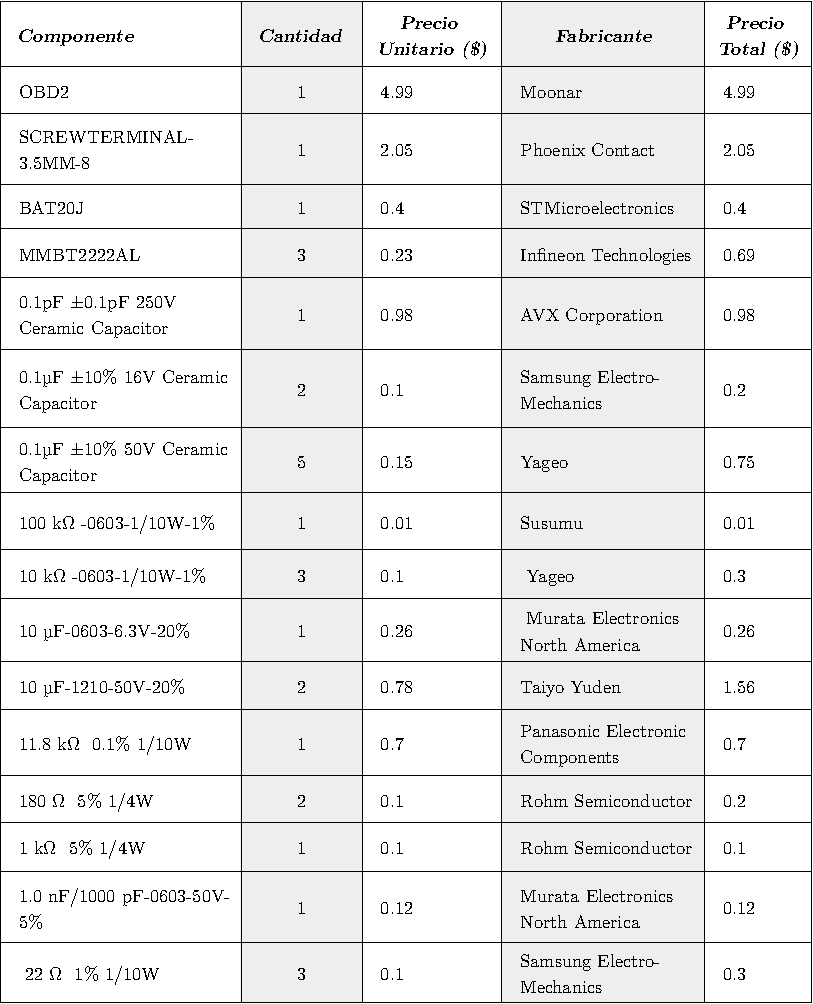
\includegraphics[width=0.9\linewidth]{BOM_1.pdf}
\end{table}

\begin{table}[htbp!]
  \centering
  \caption{Costo de componentes electrónicos (parte 2)}
  \label{diag:costos_elec_2}
  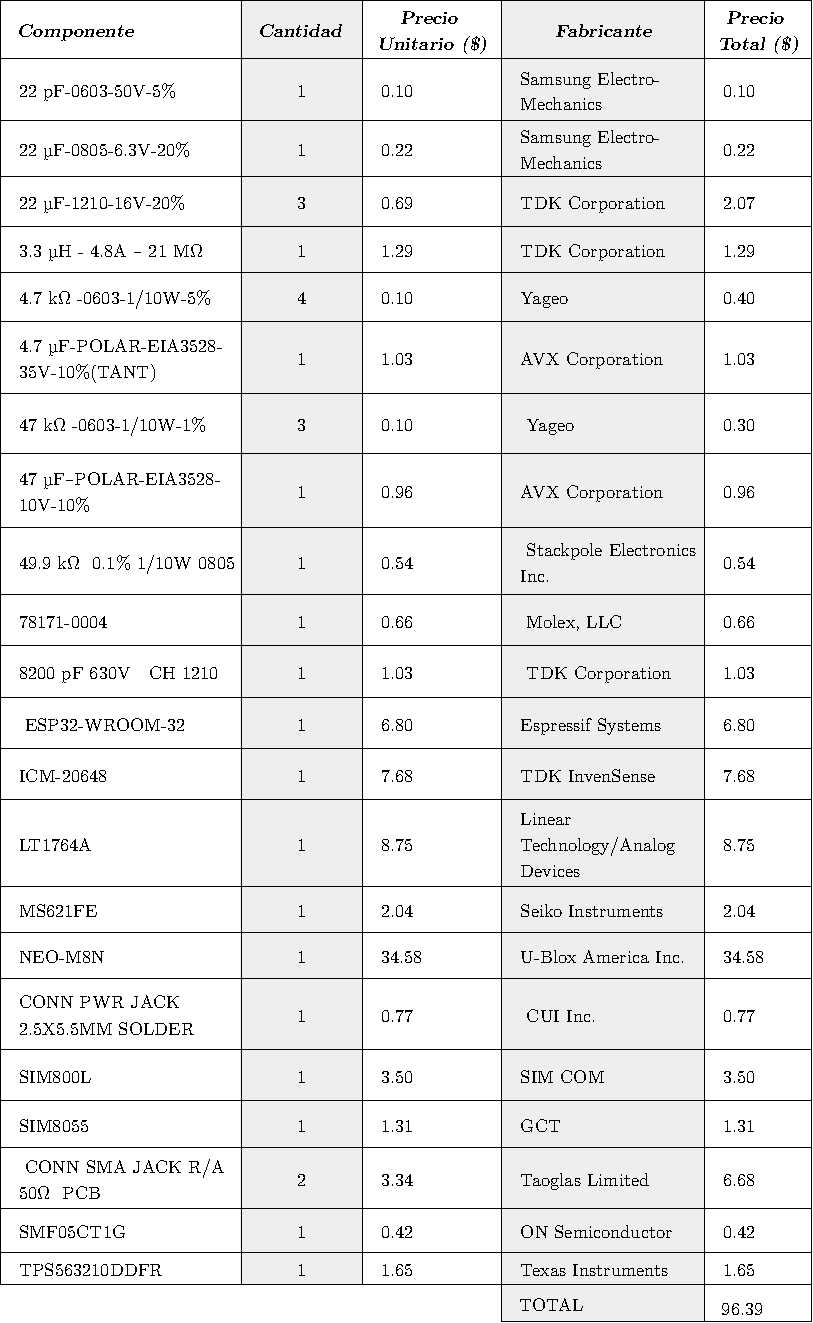
\includegraphics[width=0.9\linewidth]{BOM_2.pdf}
\end{table}

\section{Costos de fabricación y componentes mecánicos}
La Tabla (PONER TABLA AQUI) muestra los costos de fabricación del case principal y el case de la pantalla, y las piezas necesarias para el ensamble del dispositivo. La impresión 3D necesaria para el case se cotizó en 3D HUBS
\section{Costo total}



\bgroup
\def\arraystretch{1}%  1 is the default, change whatever you need
\begin{table}[htbp!]
\centering
\caption[Datos a enviar con su tamaño en bytes]{Datos a enviar con su tamaño en bytes.}
\begin{tabular}{ll}
\toprule
Datos & Tamaño en bytes \\ \midrule
Tiempo en ms & 8 \\
Aceleración frontal & 6 \\
Aceleración lateral & 6 \\
Yaw & 6 \\
Latitud & 9 \\
Longitud & 9 \\
Velocidad & 6 \\
RPM & 6 \\
Carácteres separadores & 9 \\ \midrule
Total & 65 \\ \bottomrule
\end{tabular}
\label{diag:datos_enviar}
\end{table}
\egroup